\documentclass[11pt,a4paper]{article}
\usepackage[T1]{fontenc}
\usepackage{lmodern,amsmath,amssymb,microtype,tikz}
\usepackage[a4paper,margin=1in]{geometry}
\usepackage{graphicx}
\graphicspath{{../../images/photometric_stereo/}{images/photometric_stereo/}}
\usepackage{hyperref}
\hypersetup{colorlinks=true,linkcolor=blue!55!black,urlcolor=blue!55!black,
  citecolor=blue!55!black,pdfauthor={Haiyi Li},
  pdftitle={From Four Lights to One Surface}}
\setlength{\parindent}{0pt}
\setlength{\parskip}{0.42em}
\numberwithin{equation}{section}
\raggedbottom
\newcommand{\ii}{\mathrm{i}}
\newcommand{\dd}{\mathrm{d}}
\DeclareMathOperator{\Div}{div}
\DeclareMathOperator{\Curl}{curl}
\title{\bfseries From Four Lights to One Surface\\[3pt]
  \large Photometric Stereo and the Frankot--Chellappa Algorithm}
\author{Haiyi Li}
\date{November 4, 2026}
\begin{document}
\maketitle

\begin{center}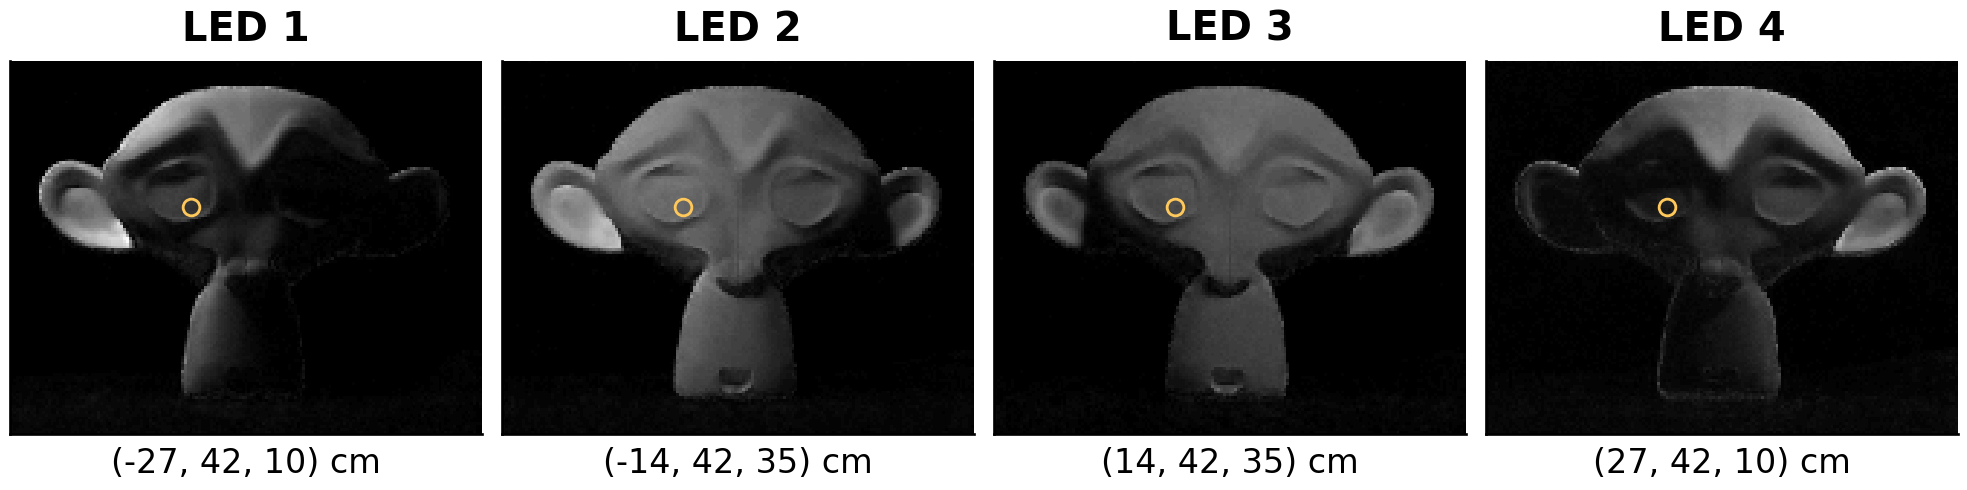
\includegraphics[width=\linewidth]{monkey_inputs.png}

\small Figure 1. Four lighting directions, one physical 3D print. Each panel shows the
same monkey head under one LED, decoded from a camera recording of the four
modulated lights. The ring marks the pixel worked through on page 2.
Cropped image data from Emma Le Francois, University of Strathclyde
\cite{data}, used under \href{https://creativecommons.org/licenses/by/4.0/}{CC BY 4.0}.
\end{center}

\section{What can four pictures tell me about one surface?}

I start by looking at the same point on the monkey's cheek in all four
pictures. The camera stayed still, so the point did too. Its brightness
changed when the lighting changed. From one dark pixel alone I could propose
dark paint, a cheek that slopes away from the light, or a shadow cast by the
brow. Across the four pictures the paint stays the same. It is the variation
in brightness with light direction that carries information about the slope.

Why should brightness tell me an angle? A small patch with area
$\dd A$ and unit normal $\mathbf n$ presents the projected area
$(\mathbf n\cdot\boldsymbol\ell_j)\,\dd A$ to a beam arriving from unit
direction $\boldsymbol\ell_j$, measured from the patch toward the light.
A patch facing the beam intercepts the most light. At grazing incidence
the projected area is zero. For a matte, diffusely reflecting surface, the
Lambertian model converts this geometric factor into measured intensity
\cite{woodham}
\begin{equation}
 I_j = a_j\,\rho\,v_j\,\max(0,\boldsymbol\ell_j\cdot\mathbf n).
 \label{eq:lambert}
\end{equation}
Here $\rho$ is the diffuse albedo of this patch and $a_j$ is the gain for
light $j$, including its strength and the common camera response scale.
The visibility $v_j$ is zero when another part of the object blocks that
light and one when the beam reaches the patch. The formula assumes
background-subtracted linear intensities.

The target is the visible surface, described by one height per image
location. First I fit a normal at each
pixel from the changing brightness, using the known lamp geometry
\cite{setup}. Then I ask whether these local tilts fit together into one
surface. That second question takes me back to my earlier work on when
a line integral gives the same answer along two different paths \cite{Li}.

\newpage
\section{Solving for the normal at one pixel}

Put the origin at the center of the printed head. Let $x$ point right,
$y$ up and $z$ toward the camera. The experiment reports four lamp positions
in centimeters relative to this origin \cite{setup}. To approximate each
lamp by a constant direction over the head, divide its position by its
distance from the origin. The four resulting row vectors form the matrix
\begin{equation}
 U=
 \operatorname{diag}\!\left(
 \frac{1}{\sqrt{2593}},\frac{1}{\sqrt{3185}},
 \frac{1}{\sqrt{3185}},\frac{1}{\sqrt{2593}}\right)
 \begin{pmatrix}
 -27&42&10\\ -14&42&35\\ 14&42&35\\ 27&42&10
 \end{pmatrix},\qquad
 L=\operatorname{diag}(a_1,a_2,a_3,a_4)\,U .
 \label{eq:measured-lights}
\end{equation}
For example, the first distance is $\sqrt{27^2+42^2+10^2}$~cm.
With the gains included, row $j$ of $L$ is $a_j\boldsymbol\ell_j^\mathsf T$.

At a front-lit, unshadowed pixel, define the three unknowns together as
$\mathbf g=\rho\mathbf n$ and stack its four intensities in $\mathbf b$.
Equation \eqref{eq:lambert} then predicts $\mathbf b=L\mathbf g$.
Measurements usually miss that equality. For a trial $\mathbf g$, vary it by
$t\mathbf h$ and differentiate the squared intensity error. At the minimum,
\begin{align}
 0&=\left.\frac{\dd}{\dd t}\,
      \tfrac12\|L(\mathbf g+t\mathbf h)-\mathbf b\|^2\right|_{t=0}
   =\mathbf h^\mathsf T L^\mathsf T(L\mathbf g-\mathbf b)
   \quad\text{for every }\mathbf h ,\nonumber\\
 L^\mathsf TL\,\widehat{\mathbf g}&=L^\mathsf T\mathbf b .
 \label{eq:photo-normal}
\end{align}
The lamp vectors span three dimensions. With positive gains,
$\mathbf h^\mathsf TL^\mathsf TL\mathbf h=\|L\mathbf h\|^2>0$ for every
$\mathbf h\ne0$, so the fit is unique. Since $\mathbf n$ has unit length,
\begin{equation}
 \widehat\rho=\|\widehat{\mathbf g}\|,\qquad
 \widehat{\mathbf n}=\widehat{\mathbf g}/\widehat\rho
 \quad(\widehat\rho>0).
 \label{eq:photo-albedo}
\end{equation}
For the displayed PNGs I take the four gains to be equal and treat the
exported grayscale levels as proportional to intensity. This is an
approximation. A common rescaling changes the scale of the fitted albedo,
while different gains for different lights can also change the normal.

Here is an actual pixel, at zero-based row 95 and column 160 of the
$219\times389$ image rectangle. Its four 8-bit display values are
$\mathbf b=(52,105,72,28)^\mathsf{T}$. Setting $a_j=1$ gives
\begin{align}
 \widehat{\mathbf g}=L^+\mathbf b&=(-30.512,20.328,118.308)^\mathsf{T},
 &\widehat\rho&=123.859,\nonumber\\
 \widehat{\mathbf n}&=(-0.2464,0.1641,0.9552)^\mathsf{T},
 & L\widehat{\mathbf g}&\simeq(56.2,96.1,80.9,23.8)^\mathsf{T}.
\end{align}
The entries of $L\widehat{\mathbf g}$ predict the four observations. Their
disagreement with $\mathbf b$ is visible even at this well-lit point.


\newpage
\section{From the normal map to two slope maps}
\begin{center}
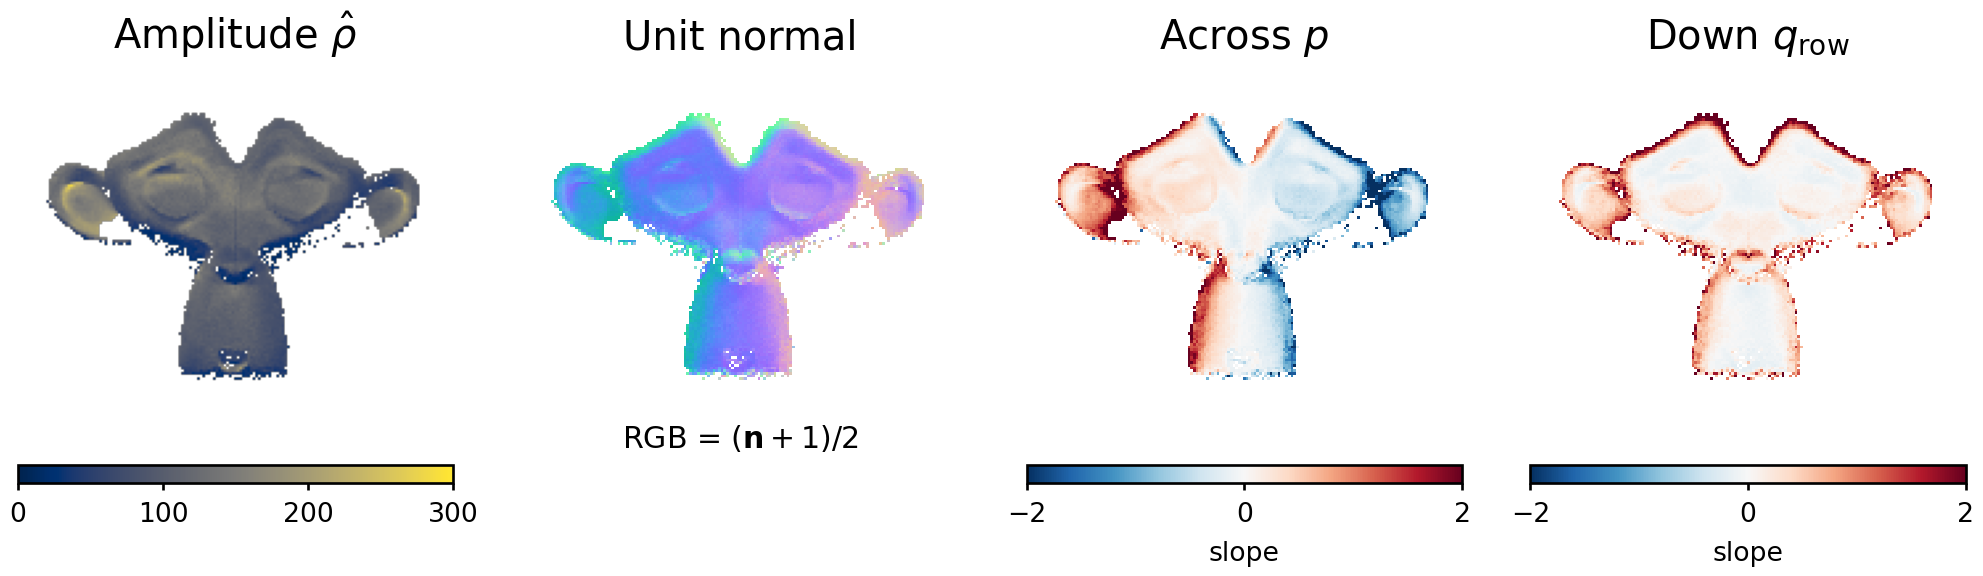
\includegraphics[width=\linewidth]{monkey_maps.png}

\small Figure 2. Fitted amplitude, unit normal and two signed slopes.
White marks pixels excluded by the rule on the last page. The slope colour
scales saturate at $\pm2$ for display. Integration uses the full retained values.
\end{center}

Suppose we view a smooth surface orthographically and write it as a height
graph $\mathbf r(x,y)=(x,y,z(x,y))$. Its two tangent vectors give a normal
by the cross product
\begin{equation}
  \mathbf r_x=(1,0,z_x),\qquad \mathbf r_y=(0,1,z_y),\qquad
  \mathbf r_x\times\mathbf r_y=(-z_x,-z_y,1).
\end{equation}
Once photometric stereo has estimated a normal $\mathbf n=(n_x,n_y,n_z)$
at a pixel, the unknown scale of the normal cancels in the ratios
\begin{equation}
  p=-\frac{n_x}{n_z},\qquad q=-\frac{n_y}{n_z},\qquad n_z\ne 0.
  \label{eq:slopes}
\end{equation}
Substituting the unit normal into \eqref{eq:lambert} gives a
\emph{reflectance map}. For one visible light it maps candidate slopes to
the predicted brightness,
\begin{equation}
 R_j(p,q)=a_j\rho\,\max\!\left(0,
 \frac{\ell_{jz}-\ell_{jx}p-\ell_{jy}q}{\sqrt{1+p^2+q^2}}\right).
\end{equation}
Increasing the row index moves down the array. With unit pixel spacing
$y=-\mathrm{row}+\mathrm{constant}$, so the array slopes are
$p=-n_x/n_z$ and $q_{\rm row}=+n_y/n_z$. At the sample pixel these are
$0.258$ and $0.172$. Moving one pixel to the right locally raises the surface
by about $0.258$ pixel units. Dividing by a small $n_z$ amplifies errors
near the silhouette.

Along any differentiable path in the original $(x,y)$ coordinates,
$\gamma(t)=(x(t),y(t))$ the chain rule would then give
\begin{equation}
  \frac{\dd}{\dd t}z(\gamma(t))
     =p(\gamma(t))x'(t)+q(\gamma(t))y'(t),\qquad
  z(P_1)-z(P_0)=\int_\gamma p\,\dd x+q\,\dd y .
  \label{eq:path}
\end{equation}

Try the measured slopes $p=0$, $q=x$ on the unit square. Walk from $(0,0)$
to $(1,1)$. Go right first, then up. Now repeat the walk in the other order.
Equation \eqref{eq:path} gives
\begin{align}
  \text{right, then up}\quad &\int_0^1 0\,\dd x+\int_0^1 1\,\dd y=1,
  \nonumber\\
  \text{up, then right}\quad &\int_0^1 0\,\dd y+\int_0^1 0\,\dd x=0.
  \label{eq:two-walks}
\end{align}
The endpoint is the same pixel. Choosing a different reference height shifts
both walks equally, so it cannot explain the discrepancy of one.

\newpage
\section{The condition I had already met}

My earlier calculation began with a path written as a graph $y=y(x)$ and
an integrand affine in the path derivative. In the notation of that note,
\begin{equation}
 S[y]=\int_a^b L(x,y,y')\,\dd x,\qquad L=A(x,y)y'+B(x,y).
\end{equation}
Compute the two terms in the Euler--Lagrange equation along a candidate
stationary path. The chain rule makes the cancellation explicit.
\begin{align}
 \frac{\partial L}{\partial y}&=A_y y'+B_y,&
 \frac{\dd}{\dd x}\frac{\partial L}{\partial y'}&=A_x+A_y y',\nonumber\\
 \frac{\partial L}{\partial y}
      -\frac{\dd}{\dd x}\frac{\partial L}{\partial y'}&=B_y-A_x .
 \label{eq:old}
\end{align}
One stationary path gives the condition $B_y-A_x=0$ along that path. Requiring
path independence throughout the domain gives a condition throughout the
domain. Indeed, take two paths from $P_0$ to $P_1$ bounding a region $D$,
with the first path followed by the reverse of the second oriented
counterclockwise. Green's theorem gives
\begin{equation}
 \int_{\gamma_1}(B\,\dd x+A\,\dd y)-\int_{\gamma_2}(B\,\dd x+A\,\dd y)
      =\iint_D(A_x-B_y)\,\dd x\,\dd y .
 \label{eq:green}
\end{equation}
For continuous derivatives, zero circulation around every small rectangle
forces $A_x-B_y=0$ at each point. A nonzero value at one point would keep
its sign on a sufficiently small rectangle about that point.

Now set $B=p$ and $A=q$. The same quantity has the name
$\Curl F=q_x-p_y$, where $F=(p,q)$. In \eqref{eq:two-walks} it equals one
everywhere, so its integral over the unit square accounts for the entire
height discrepancy. On a simply connected planar domain, a $C^1$ field
with zero curl has path-independent integrals. Fix $P_0$ and define
\begin{equation}
 z(x,y)=z(P_0)+\int_{P_0}^{(x,y)}p\,\dd x+q\,\dd y .
 \label{eq:potential}
\end{equation}
Append a horizontal segment of length $h$ to the integration path. Then
$[z(x+h,y)-z(x,y)]/h=h^{-1}\int_x^{x+h}p(s,y)\,\dd s\to p(x,y)$.
A vertical segment gives $z_y=q$. This constructs the height from exact slopes.

My earlier note continued with $g=A+\ii B$. The first Cauchy--Riemann
equation is $A_x=B_y$. The second would impose $A_y=-B_x$, hence
$\Delta z=q_y+p_x=0$. Height recovery only needs the first condition.
For instance $z=x^2+y^2$ gives $p=2x$, $q=2y$. All paths agree, although
$\Delta z=4$.

\newpage
\section{Fitting a surface when the walks disagree}

This time the unknown is a function on the image. Given both measured
slopes, choose the height whose gradient has the smallest integrated squared
discrepancy. The factor $\tfrac12$ simplifies the variation. Write
\begin{equation}
 E[z]=\tfrac12\int_\Omega\big[(z_x-p)^2+(z_y-q)^2\big]\,\dd x\,\dd y
     =\tfrac12\int_\Omega|\nabla z-F|^2\,\dd x\,\dd y .
 \label{eq:energy}
\end{equation}
For an admissible perturbation $\eta$, substitute $z+\varepsilon\eta$.
Expanding both squares gives the exact change
\begin{align}
 E[z+\varepsilon\eta]-E[z]
 &=\varepsilon\int_\Omega[(z_x-p)\eta_x+(z_y-q)\eta_y]
   +\tfrac{\varepsilon^2}{2}\int_\Omega|\nabla\eta|^2 . \label{eq:variation}
\end{align}
Area measure is understood in domain integrals below. At a minimiser the
coefficient of $\varepsilon$ vanishes for every such $\eta$. It says that
the residual slope is orthogonal in $L^2$ to every admissible gradient.
Conversely, once this coefficient vanishes, the remaining square in
\eqref{eq:variation} proves minimality. Equal energies then require
$\nabla\eta=0$, so on a connected domain the freedom is an additive constant
when the reference height is free.

To see which equation we must solve, integrate the two terms separately.
For smooth fields and an outward unit normal $\nu=(\nu_x,\nu_y)$,
\begin{align}
 \int_\Omega(z_x-p)\eta_x
  &=-\int_\Omega(z_{xx}-p_x)\eta
    +\int_{\partial\Omega}(z_x-p)\nu_x\eta\,\dd s,\nonumber\\
 \int_\Omega(z_y-q)\eta_y
  &=-\int_\Omega(z_{yy}-q_y)\eta
    +\int_{\partial\Omega}(z_y-q)\nu_y\eta\,\dd s .
\end{align}
Taking $\eta$ supported inside the domain eliminates the boundary terms.
The remaining integral is zero for every such $\eta$, giving Poisson's equation
\begin{equation}
 \boxed{\Delta z=p_x+q_y=\Div F.} \label{eq:poisson}
\end{equation}
If the boundary height is free, arbitrary boundary variations also give
$(\nabla z-F)\cdot\nu=0$. If the height is fixed there, $\eta=0$ there.
For the Fourier construction we instead identify opposite sides of a
rectangle and fit a periodic height. Periodic variations make opposite
boundary terms cancel for smooth periodic data.

Why does \eqref{eq:poisson} contain divergence when curl detected the
problem? Curl measures the disagreement between paths. The minimisation
imposes $\Div(F-\nabla z)=0$ on the slope left over, which gives divergence
on the right-hand side of the equation for the height.

\newpage
\section{Why does differentiation become multiplication?}

The step I want to understand is the appearance of the frequency in place of a
derivative. Start in one dimension with the convention
$\widehat g(\xi)=\int_{\mathbb R}g(t)e^{-\mathrm i\xi t}\,\mathrm dt$.
Suppose $g$ is continuously differentiable, $g$ and $g'$ are integrable,
and $g(t)\to0$ at both ends of the line. Integrating by parts gives
\begin{equation}
  \widehat{g'}(\xi)
  =\bigl[g(t)e^{-\mathrm i\xi t}\bigr]_{-\infty}^{\infty}
     -\int_{\mathbb R}g(t)(-\mathrm i\xi)e^{-\mathrm i\xi t}\,\mathrm dt
  =\mathrm i\xi\,\widehat g(\xi).
\end{equation}
The boundary term vanishes by decay. The two minus signs have different
origins. One comes from integration by parts and the other from differentiating
the exponential in the transform. Their product accounts for the positive sign.

For the rectangular image model, let $Q=[0,L_x]\times[0,L_y]$ and write
$\boldsymbol{x}=(x,y)$. Take $f$ to be a smooth periodic height field with these
two periods. For integers $m,n$ define
\begin{equation}
  k=(k_x,k_y)=\left(\frac{2\pi m}{L_x},\frac{2\pi n}{L_y}\right),
  \qquad
  \widehat f(k)=\frac{1}{|Q|}\int_Q
        f(\boldsymbol{x})e^{-\mathrm ik\cdot\boldsymbol{x}}\,\mathrm d\boldsymbol{x} .
\end{equation}
This time there is no decay to invoke. Hold $y$ fixed and integrate first in
$x$. The endpoint contribution before integration in $y$ is
\begin{equation}
  \bigl[f(x,y)e^{-\mathrm i(k_xx+k_yy)}\bigr]_{x=0}^{L_x}
  =e^{-\mathrm i k_y y}\bigl(f(L_x,y)e^{-2\pi\mathrm i m}-f(0,y)\bigr)=0 .
\end{equation}
The heights agree at opposite edges, and the exponential completes an integer
number of turns. In detail, with $E=e^{-\ii(k_xx+k_yy)}$ and
$\partial_x E=-\ii k_x E$, the remaining integral is
\begin{align}
 \widehat{\partial_x f}(k)
 &=\frac{1}{|Q|}\int_0^{L_y}
    \left([fE]_{x=0}^{L_x}-\int_0^{L_x}f\,\partial_x E\,\dd x\right)\dd y
   =\frac{\ii k_x}{|Q|}\int_Q fE\,\dd x\,\dd y .
\end{align}
In the $y$ direction, $f(x,L_y)=f(x,0)$ and
$e^{-2\pi\mathrm i n}=1$ cancel the other pair of edges. Thus
\begin{equation}\label{eq:multiplier}
  \widehat{\partial_x f}(k)=\mathrm i k_x\widehat f(k),
  \qquad
  \widehat{\partial_y f}(k)=\mathrm i k_y\widehat f(k).
\end{equation}
Differentiate twice and add. Each second derivative brings in a factor of
$\mathrm i^2=-1$, giving
\begin{equation}\label{eq:lapmult}
  \widehat{\Delta f}(k)
  =-(k_x^2+k_y^2)\widehat f(k)
  =-|k|^2\widehat f(k).
\end{equation}
At $k=0$ this factor vanishes. That mode records the mean height,
which a measurement of slopes cannot determine.

\newpage
\section{Recovering one height coefficient at a time}

Take Fourier coefficients of both sides of \eqref{eq:poisson} on the periodic
rectangle $Q$. Write $P=\widehat p(k)$, $U=\widehat q(k)$ and
$Z=\widehat z(k)$ at the current frequency. By \eqref{eq:multiplier}
and \eqref{eq:lapmult},
\begin{equation}
 -(k_x^2+k_y^2)Z=\ii k_xP+\ii k_yU,\qquad
 \boxed{Z=\frac{-\ii(k_xP+k_yU)}{k_x^2+k_y^2}}\quad(k\ne0).
 \label{eq:fc}
\end{equation}
Knowing the coefficients gives the height by synthesis,
$z(x,y)=\sum_{m,n\in\mathbb Z}\widehat z(k)e^{\ii(k_x x+k_y y)}$.
At $k=0$ the equation reads $0=0$. Setting $Z(0)=0$ chooses a surface of
mean height zero. There is a separate issue with the \emph{slopes} at zero
frequency. Every periodic gradient has zero mean, since integrating either
partial derivative over its period gives the difference of equal endpoint
values. A uniform tilt $F=(1,0)$ therefore projects to zero on the torus.
On an ordinary rectangle its exact height is $z=x+C$.

We can also derive \eqref{eq:fc} directly from the two slope measurements.
Orthogonality of the Fourier modes (Parseval's identity) rewrites
\eqref{eq:energy} as a sum of independent squared errors,
\begin{equation}
 \frac{2E[z]}{|Q|}=\sum_k\big(
   |\ii k_x Z-P|^2+|\ii k_y Z-U|^2\big).
\end{equation}
At one nonzero frequency put $a=(\ii k_x,\ii k_y)^\mathsf{T}$,
$b=(P,U)^\mathsf{T}$, $K=a^*a=k_x^2+k_y^2$, and $c=a^*b$.
Here $^*$ denotes conjugate transpose. Expanding and completing the square gives
\begin{align}
 \|aZ-b\|^2
 &=K|Z|^2-\overline Zc-Z\overline c+b^*b \nonumber\\
 &=K|Z-c/K|^2+b^*b-|c|^2/K .
 \label{eq:square}
\end{align}
The minimum is at $Z=c/K$. Conjugating the two entries of $a$ gives
$c=-\ii k_xP-\ii k_yU$, including the minus sign in \eqref{eq:fc}.
For real data the solutions at $k$ and $-k$ are conjugates, so their inverse
Fourier series gives a real height.

What happened to the slopes? Multiplying $Z$ by $a$ gives their fitted values,
\begin{equation}
 \widehat{\nabla z}(k)
 =\frac{1}{k_x^2+k_y^2}
 \begin{pmatrix}k_x^2&k_xk_y\\ k_xk_y&k_y^2\end{pmatrix}
 \begin{pmatrix}P\\U\end{pmatrix}
 =\frac{k k^\mathsf{T}}{|k|^2}\,b .
 \label{eq:projector}
\end{equation}
Each allowed slope amplitude lies along $k$. The matrix keeps that component
of $b$ and removes the perpendicular one. This orthogonal projection onto
integrable slopes is the construction of Frankot and Chellappa \cite{FC}.

\newpage
\section{Two waves and a height I can check by hand}

On the square $[0,2\pi]^2$ with opposite edges identified, suppose the measured
slopes are
\begin{equation}
 F=(p,q)=(3,1)\cos s+(-1,3)\cos t,\qquad s=x+y,\quad t=2x-y .
 \label{eq:two-waves}
\end{equation}
Can I integrate the first wave alone? For a height $b\sin s$, the two slopes
would both be $b\cos s$. The observations ask for $b=3$ and $b=1$ at the
same time. Their squared disagreement is
$(b-3)^2+(b-1)^2=2(b-2)^2+2$. The closest choice is $b=2$.
The picture shows the calculation in the plane of slope amplitudes.

\begin{center}
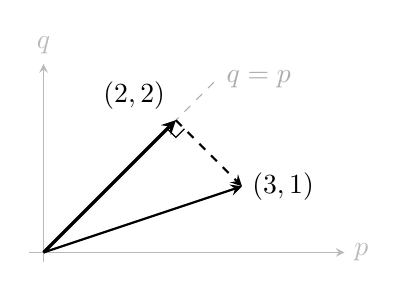
\begin{tikzpicture}[>=stealth,scale=0.84]
  \draw[gray!55,->] (-.22,0) -- (4.55,0) node[right] {$p$};
  \draw[gray!55,->] (0,-.15) -- (0,2.85) node[above] {$q$};
  \draw[gray!65,dashed] (0,0) -- (2.62,2.62) node[right] {$q=p$};
  \draw[very thick,->] (0,0) -- (2,2) node[above left] {$(2,2)$};
  \draw[thick,->] (0,0) -- (3,1) node[right] {$(3,1)$};
  \draw[thick,dashed,->] (2,2) -- (3,1);
  \draw (1.87,1.87) -- (2,1.74) -- (2.13,1.87);
\end{tikzpicture}
\end{center}

The second wave has a different direction. A height $c\sin t$ contributes
$(2c,-c)\cos t$. The integral of $\cos s\cos t$ is zero because the two
wavevectors are distinct up to sign, so we can choose $c$ independently.
For this wave the squared disagreement becomes
\begin{equation}
 (2c+1)^2+(-c-3)^2=5c^2+10c+10=5(c+1)^2+5 .
\end{equation}
Thus $c=-1$. Every other nonconstant height mode would introduce a gradient
at a frequency absent from the data and increase the error. The mean-zero
height, its gradient and the residual are therefore
\begin{align}
 z_* &= 2\sin s-\sin t, &
 \nabla z_* &= (2,2)\cos s+(-2,1)\cos t, \notag\\
 F-\nabla z_* &= (1,-1)\cos s+(1,2)\cos t . &&
 \label{eq:two-wave-residual}
\end{align}
Indeed, $(1,-1)\cdot(1,1)=0$ and $(1,2)\cdot(2,-1)=0$.
Differentiating the data and the height gives a second check on the signs,
\begin{equation}
 \partial_x p+\partial_y q=-4\sin s+5\sin t=\Delta z_* .
\end{equation}
Both squared cosines average to $1/2$. The mean squared residual is therefore
$(2+5)/2=7/2$. One feature of the result is easy to miss. If an instrument
also adds $\varepsilon(1,1)\cos s$, the extra term is already the gradient
of $\varepsilon\sin s$. The reconstructed height changes by exactly that
amount. Integrability alone cannot distinguish this error from a real ripple.

\newpage
\section{What changes on a pixel grid?}

Take $N_x$ by $N_y$ pixels with spacings $h_x,h_y$ and periodic indices
$j,\ell$ starting at zero. At frequency indices $m,n$, write
$\theta_x=k_xh_x=2\pi m/N_x$ and $\theta_y=k_yh_y=2\pi n/N_y$. The
discrete Fourier transform (DFT) uses the phase
$e^{-\ii(j\theta_x+\ell\theta_y)}$. Set $S_x^+ f_{j,\ell}=f_{j+1,\ell}$.
Changing the summation index to $r=j+1$ gives
\begin{align}
 \widehat{S_x^+ f}
 &=\sum_{j,\ell} f_{j+1,\ell}e^{-\ii(j\theta_x+\ell\theta_y)}
   =\sum_{r,\ell} f_{r,\ell}e^{-\ii((r-1)\theta_x+\ell\theta_y)}
   =e^{\ii\theta_x}\widehat f . \label{eq:dft-shift}
\end{align}
The wrap from $r=N_x$ to $r=0$ is valid because $f$ is periodic and
$e^{-\ii N_x\theta_x}=1$. A backward shift gives $e^{-\ii\theta_x}$.
For the centered difference $D_x=(S_x^+-S_x^-)/(2h_x)$, subtraction gives
\begin{equation}
 \widehat{D_x f}
 =\frac{e^{\ii\theta_x}-e^{-\ii\theta_x}}{2h_x}\widehat f
 =\frac{\ii\sin\theta_x}{h_x}\widehat f
 =d_x\widehat f,\qquad d_y=\frac{\ii\sin\theta_y}{h_y} .
 \label{eq:centered-symbol}
\end{equation}
This is the centered-difference choice in Section IV-A of \cite{FC}.
For a fixed physical $k_x$, $\sin(k_xh_x)/h_x$ tends to $k_x$
as the spacing tends to zero. At finite spacing the choice of derivative
determines which multiplier belongs in the reconstruction.

For one frequency let $Z$ be the unknown height coefficient. Its two
predicted slopes are $d_xZ,d_yZ$. Orthogonality of the least-squares
residual to the complex vector $(d_x,d_y)$ gives
\begin{align}
 \overline{d_x}(d_xZ-\widehat p)+\overline{d_y}(d_yZ-\widehat q)&=0,
 \notag\\
 Z&=\frac{\overline{d_x}\,\widehat p+\overline{d_y}\,\widehat q}
               {|d_x|^2+|d_y|^2}
 \qquad (|d_x|^2+|d_y|^2>0). \label{eq:discrete-recovery}
\end{align}
The bar denotes complex conjugation. To run the algorithm, take the
two-dimensional FFT of each slope image, apply \eqref{eq:discrete-recovery}
at every frequency with a positive denominator, then inverse transform the
height coefficients. Set jointly invisible coefficients to zero before the
inverse transform to select the minimum-norm height.

The constant mode is always invisible. On an even $x$ grid the alternating
sequence $(-1)^j$ is invisible to $D_x$ as well, since its two neighbours
are equal. When both grid sizes are even, the zero denominator occurs at all
four phase pairs in $\{0,\pi\}^2$. A single vanishing multiplier still
leaves a usable estimate whenever the other one is nonzero.

\newpage
\section{Back to the four lights}
\begin{center}
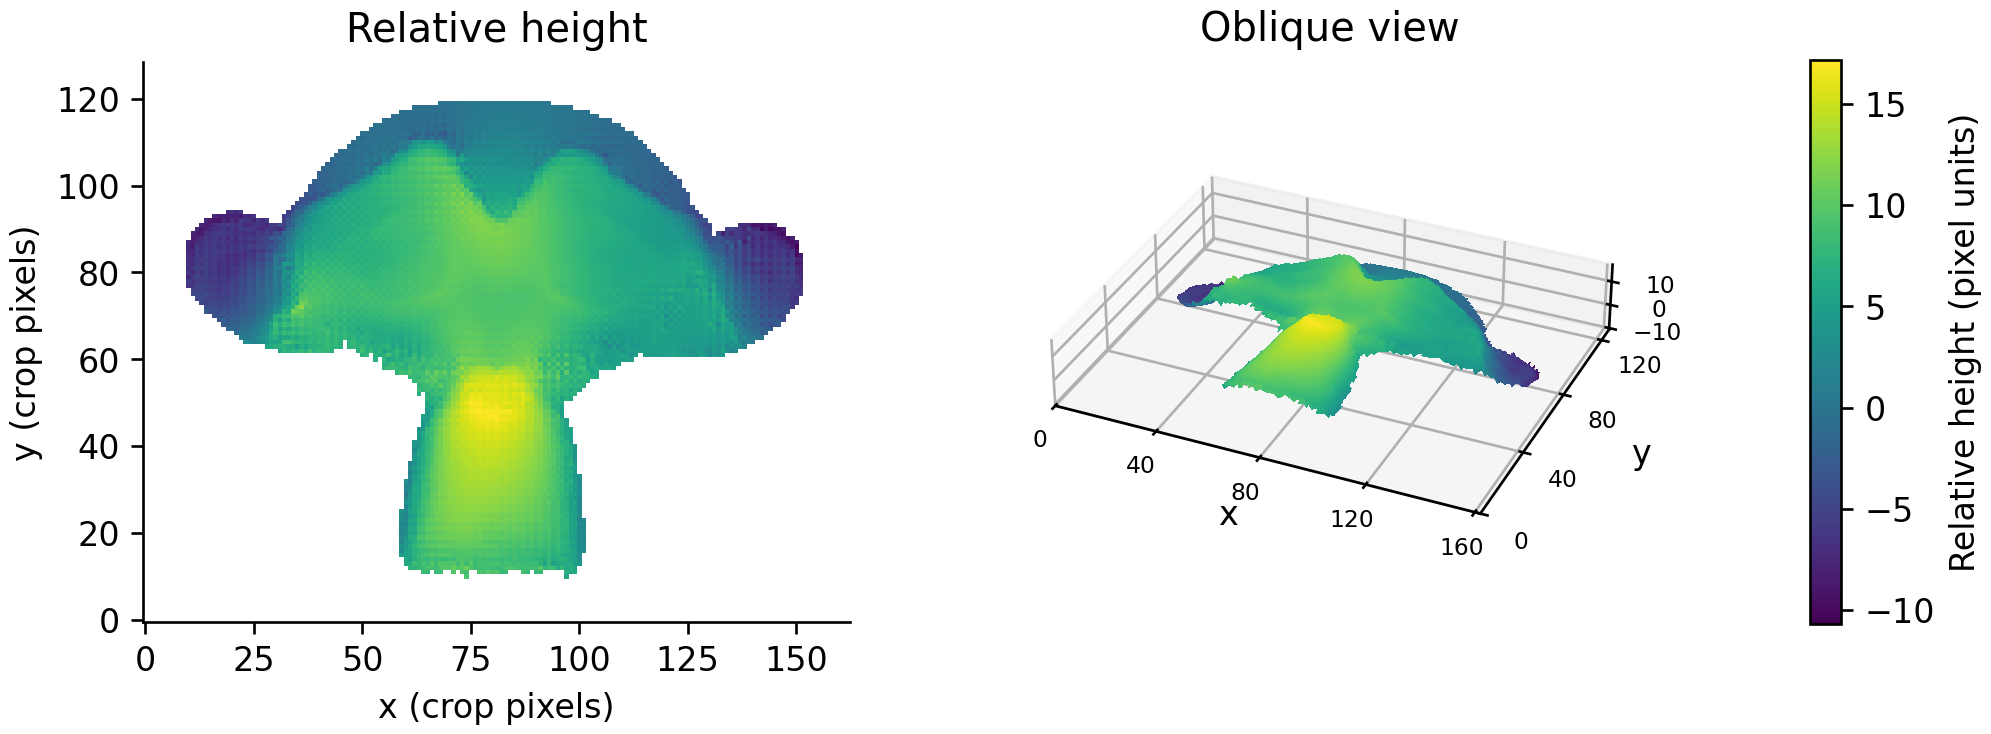
\includegraphics[width=.96\linewidth]{monkey_surface.png}

\small Figure 3. The mean-zero FC height field from the four lighting
channels, viewed from the front and at an angle. The axes use pixel units.
\end{center}

To reproduce this surface, take the common $219\times389$ image rectangle
from the four exports. Within rows $[45,174)$ and columns $[98,261)$,
threshold the brightest of the four images at 18 grey levels. Keep the
largest four-connected component and fill its holes. This estimates a
silhouette of 8,168 pixels. I retain slopes where $\widehat n_z\ge0.2$ and
at least three of the four intensities are at least 8. This leaves 6,285
pixels. The thresholds are choices for this demonstration. Each retained
normal uses all four observations with equal weights.

I assign zero slopes everywhere else, including excluded pixels inside the
silhouette. I then apply the centered-difference formula
\eqref{eq:discrete-recovery} to the whole rectangle, with periodic edges,
unit spacing and zero mean height. Thus the boundary and missing pixels
affect the fitted surface. The silhouette is used again to display the
result. The two ears separate in the height map, but their height relative
to the face depends on how the intervening slopes were filled. No back
surface or physical depth scale is recovered.

One check is to differentiate the height again with the same centered
differences. Relative to a flat surface, the ratio of squared slope errors is
\begin{equation}
 \frac{\sum[(D_x z-p)^2+(D_{\rm row}z-q_{\rm row})^2]}
      {\sum[p^2+q_{\rm row}^2]}=0.3491
\end{equation}
over the full rectangle. This measures the slope fit. The experimenters used
fast marching to integrate their normals \cite{setup}. The height in Figure 3
comes from our own brightness fit and Fourier integration.

My earlier question was whether two paths give the same height difference.
At the cheek pixel the camera supplied four brightnesses, and a fit supplied
two slopes. It took a second fit, across pixels, to give those slopes a
single surface to live on.

\newpage
\section*{Repeating the calculation}

The \href{https://github.com/Gatsby0916/math-thoughts/blob/main/latex/photometric_stereo/reconstruct.py}{companion Python script}
reads the four LED images directly from the
\href{https://pure.strath.ac.uk/ws/portalfiles/portal/99603607/Out_of_plane_configuration_monkey_head.zip}{monkey-head archive}
and verifies its SHA-256 digest. With NumPy, SciPy, Pillow and Matplotlib
installed, run the following in the directory containing the script, with
the archive alongside it or with its full path as the argument.
\begin{verbatim}
python reconstruct.py Out_of_plane_configuration_monkey_head.zip
\end{verbatim}
The script prints the example pixel, the number of usable slopes and the
squared-error ratio. It writes the three figures to the repository's
image directory. The essential arrays can also be traced by their shapes.
\begin{enumerate}
\item \textbf{Four observations per point.} For each released display export
take rows $[93,312)$ and columns $[65,454)$, excluding margins and colour
bars. The result has 219 rows and 389 columns. Stacking the four pictures
in LED order gives an array of shape $(219,389,4)$. All four use the
same mapping of the authors' displayed range $[0,200]$ to 8-bit grey.
\item \textbf{Three fitted components per point.} The $4\times3$ lighting
matrix has a $3\times4$ pseudoinverse. Multiplying each column of four
intensities by it yields three components of $\widehat{\mathbf g}$.
Their length gives the amplitude map. Their direction gives the normal map.
\item \textbf{Two slopes to one height.} Form the two $219\times389$ slope
images and apply a 2D FFT to each. At each frequency, equation
\eqref{eq:discrete-recovery} combines their coefficients into one height
coefficient. An inverse 2D FFT gives the $219\times389$ height image.
Both dimensions here are odd, so the constant is the only jointly invisible mode.
\end{enumerate}
To recompile the note in the repository, work in
\path{latex/photometric_stereo} and run
\texttt{latexmk -pdf frankot\_chellappa.tex}.

\begin{thebibliography}{5}
\bibitem{data} E. Le Francois, M. Dawson, M. Strain and J. Herrnsdorf.
\href{https://doi.org/10.15129/44b337ab-9fd9-4983-9079-a0dcfaae1d84}{Data for
Synchronization-Free Top-down Illumination Photometric Stereo Imaging Using Light-Emitting Diodes and a Mobile Device}.
University of Strathclyde (2020), out-of-plane monkey-head capture.
Figures 1--3 are crops and computations using these data under
\href{https://creativecommons.org/licenses/by/4.0/}{CC BY 4.0}.
\bibitem{setup} E. Le Francois et al.
\href{https://doi.org/10.1364/OE.408658}{Synchronization-free top-down illumination photometric stereo imaging using light-emitting diodes and a mobile device}.
\emph{Optics Express} \textbf{29} (2021), 1502--1515.
\bibitem{woodham} R. J. Woodham.
\href{https://doi.org/10.1117/12.7972479}{Photometric method for determining surface orientation from multiple images}.
\emph{Optical Engineering} \textbf{19} (1980), 139--144.
\bibitem{Li} H. Li. \href{https://github.com/Gatsby0916/math-thoughts/blob/main/markdown/2026-10-07_variational_path_to_laplace.md}{A Variational Path to Laplace's Equation via Complex Analysis}.
  \emph{Math Thoughts}, October 7, 2026.
\bibitem{FC} R. T. Frankot and R. Chellappa.
  \href{https://doi.org/10.1109/34.3909}{A method for enforcing integrability in shape from shading algorithms}.
  \emph{IEEE Transactions on Pattern Analysis and Machine Intelligence}
  \textbf{10} (1988), 439--451.
\end{thebibliography}
\end{document}
